\section{Thực nghiệm và thảo luận} % Section 4

\subsection{Thiết lập thực nghiệm} % Section 4.1

Trong phần này, chúng tôi tiến hành đánh giá hiệu suất của hai mô hình học sâu là \textbf{MobileNetV3Small} và \textbf{ResNet18} trong bài toán phân loại cảm xúc khuôn mặt trên tập dữ liệu FER2013. Mỗi mô hình được thử nghiệm trên ba biến thể của tập dữ liệu nhằm khảo sát khả năng thích nghi với điều kiện ánh sáng thay đổi và hiệu quả của các kỹ thuật tăng cường dữ liệu.

\begin{table}[H]
\centering
\caption{Kiến trúc mô hình MobileNetV3Small sử dụng trong thực nghiệm}
\begin{tabular}{@{}lll@{}}
\toprule
\textbf{Layer (type)} & \textbf{Output Shape} & \textbf{Param \#} \\ \midrule
MobileNetV3Small (Functional)   & (None, 7, 7, 576) & 939,120 \\
GlobalAveragePooling2D          & (None, 576)       & 0       \\
Dense (128 units)               & (None, 128)       & 73,856  \\
Dropout                         & (None, 128)       & 0       \\
Dense (64 units)                & (None, 64)        & 8,256   \\
Dropout                         & (None, 64)        & 0       \\
Dense (7 units - output)        & (None, 7)         & 455     \\ \bottomrule
\end{tabular}
\label{tab:model-architecture}
\end{table}

Bảng~\ref{tab:model-architecture} mô tả kiến trúc của mô hình MobileNetV3Small được sử dụng trong thực nghiệm. Mô hình gốc MobileNetV3Small được sử dụng như một bộ trích xuất đặc trưng (feature extractor) đầu vào với đầu ra có kích thước \texttt{(7, 7, 576)}. Sau đó, lớp \texttt{GlobalAveragePooling2D} được áp dụng để giảm chiều không gian, tạo vector đặc trưng một chiều với 576 phần tử.

Tiếp theo là hai lớp \texttt{Dense} với số lượng đơn vị lần lượt là 128 và 64, đi kèm với các lớp \texttt{Dropout} nhằm giảm hiện tượng overfitting. Cuối cùng, lớp \texttt{Dense} đầu ra có 7 đơn vị tương ứng với 7 lớp cảm xúc cần phân loại.

Tổng số tham số huấn luyện của toàn bộ mô hình là khoảng 1 triệu, trong đó phần lớn nằm ở MobileNetV3Small. Việc sử dụng kiến trúc gọn nhẹ giúp mô hình đạt được hiệu quả cao mà vẫn đảm bảo tốc độ xử lý nhanh, phù hợp với các ứng dụng thực tế như trên thiết bị di động.


\subsection{Biểu đồ, bảng biểu, hình ảnh minh hoạ} % Section 4.2

\subsubsection{MobileNetV3Small}

\begin{table}[H]
\centering
\caption{Độ chính xác của các phiên bản mô hình MobileNetV3Small trên tập dữ liệu FER2013}
\begin{tabular}{@{}lc@{}}
\toprule
\textbf{Tên kiến trúc} & \textbf{Độ chính xác (\%)} \\ \midrule
MobileNetV3Small + FER2013 & 61.63 \\
MobileNetV3Small + FER2013 (Low Light Images - LLI) & 58.86 \\
MobileNetV3Small + FER2013 (LLI + adaptive augmentation) & 61.55 \\ \bottomrule
\end{tabular}
\label{tab:training-results}
\end{table}

Bảng~\ref{tab:training-results} trình bày độ chính xác khi huấn luyện mô hình MobileNetV3Small trên các phiên bản khác nhau của tập dữ liệu FER2013. Trong đó, FER2013 là tập dữ liệu gốc chứa các hình ảnh khuôn mặt thể hiện cảm xúc. 

Khi huấn luyện trên tập FER2013 gốc, mô hình đạt độ chính xác cao nhất là 61.63\%. Việc mô phỏng điều kiện ánh sáng yếu thông qua tập dữ liệu LLI làm giảm độ chính xác mô hình, phản ánh thách thức trong việc nhận diện cảm xúc dưới điều kiện chiếu sáng kém, giảm còn 58.86\%. Tuy nhiên, khi kết hợp LLI với phương pháp tăng cường dữ liệu thích ứng (adaptive augmentation), độ chính xác cải thiện đáng kể lên 61.55\%, gần tương đương với mô hình gốc. 

Điều này cho thấy rằng các kỹ thuật tăng cường dữ liệu phù hợp có thể giúp mô hình thích nghi tốt hơn với điều kiện ánh sáng kém, nhưng cần được áp dụng và điều chỉnh một cách hợp lý để tránh làm nhiễu thông tin đầu vào.
% \begin{figure}[H]
% \centering
% 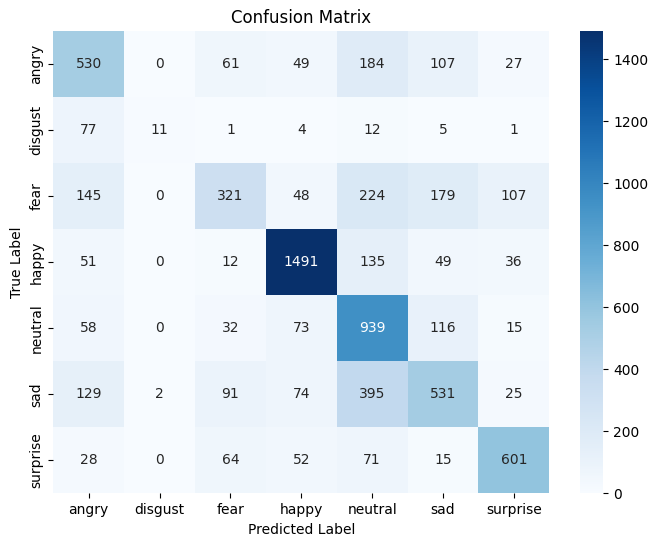
\includegraphics[width=1\textwidth]{img/confusionMatrixMobilenetV3.png}  % thay bằng tên file ảnh
% \caption{Ma trận nhầm lẫn}
% \end{figure}


\begin{figure}[H]
\centering
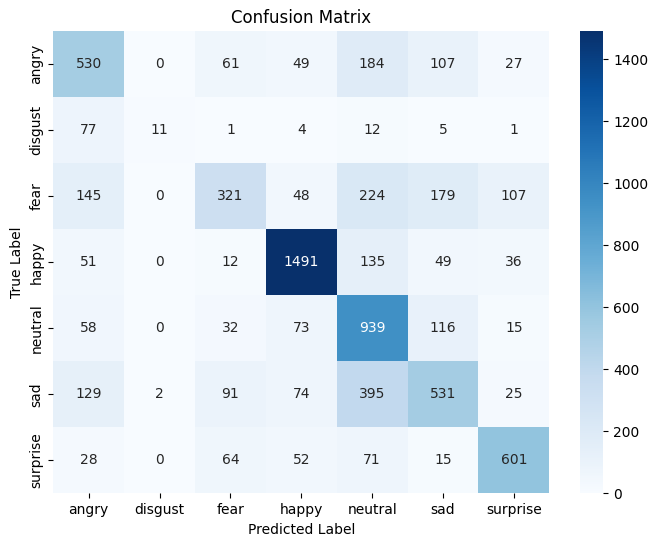
\includegraphics[width=1\textwidth]{img/confusionMatrixMobilenetV3.png}
\caption{Ma trận nhầm lẫn trên tập kiểm tra của mô hình MobileNetV3}
\label{fig:confusion-mobilenetv3}
\end{figure}

Hình~\ref{fig:confusion-mobilenetv3} trình bày ma trận nhầm lẫn của mô hình \textbf{MobileNetV3} trong nhiệm vụ phân loại cảm xúc khuôn mặt. Kết quả cho thấy mô hình nhận diện tốt các cảm xúc có đặc trưng rõ ràng như:

\begin{itemize}
    \item \textbf{Happy}: có \textbf{1,491} mẫu được dự đoán đúng (\textbf{95.40\%}).
    \item \textbf{Neutral}: có \textbf{939} mẫu đúng (\textbf{64.22\%}).
    \item \textbf{Surprise}: đạt \textbf{601} mẫu đúng (\textbf{86.48\%}).
\end{itemize}

Tuy nhiên, hiệu suất giảm đáng kể với các cảm xúc khó phân biệt hơn:

\begin{itemize}
    \item \textbf{Disgust}: chỉ \textbf{11} mẫu được nhận diện đúng (\textbf{21.57\%}), trong khi bị nhầm sang \textbf{Angry} tới \textbf{28} mẫu (\textbf{54.90\%}).
    
    \item \textbf{Fear}: chỉ \textbf{42} mẫu đúng (\textbf{8.57\%}), trong khi bị nhầm với:
    \begin{itemize}
        \item \textbf{Neutral}: \textbf{224} mẫu (\textbf{45.71\%})
        \item \textbf{Sad}: \textbf{179} mẫu (\textbf{36.53\%})
        \item \textbf{Angry}: \textbf{145} mẫu (\textbf{29.59\%})
    \end{itemize}

    \item \textbf{Sad}: chỉ \textbf{107} mẫu đúng (\textbf{17.63\%}), bị nhầm với:
    \begin{itemize}
        \item \textbf{Neutral}: \textbf{395} mẫu (\textbf{65.07\%})
        \item \textbf{Fear}: \textbf{91} mẫu (\textbf{14.98\%})
    \end{itemize}
\end{itemize}

Tổng thể, ma trận nhầm lẫn cung cấp cái nhìn rõ nét về khả năng mô hình phân biệt giữa các cảm xúc. Trong khi các cảm xúc tích cực như \textit{happy} và \textit{surprise} đạt hiệu suất cao, các cảm xúc tiêu cực như \textit{fear}, \textit{sad} và \textit{disgust} dễ bị nhầm lẫn lẫn nhau, đòi hỏi cải tiến thêm về dữ liệu huấn luyện và biểu diễn đặc trưng.

\subsubsection{ResNet18}

\begin{table}[H]
\centering
\caption{Độ chính xác của các phiên bản mô hình ResNet18 trên tập dữ liệu FER2013}
\begin{tabular}{@{}lc@{}}
\toprule
\textbf{Tên kiến trúc} & \textbf{Độ chính xác (\%)} \\ \midrule
ResNet18 + FER2013 & 67.23 \\
ResNet18 + FER2013 (Low Light Images - LLI) & 67.04 \\
ResNet18 + FER2013 (LLI + adaptive augmentation) & 67.48 \\ \bottomrule
\end{tabular}
\label{tab:resnet-results}
\end{table}


Bảng~\ref{tab:resnet-results} thể hiện độ chính xác của mô hình ResNet18 khi huấn luyện trên các phiên bản khác nhau của tập dữ liệu FER2013. Tương tự như mô hình MobileNetV3Small, FER2013 là tập dữ liệu ảnh khuôn mặt thể hiện cảm xúc.

Mô hình ResNet18 huấn luyện trên tập FER2013 gốc đạt độ chính xác cao nhất là 67.23\%. Khi sử dụng phiên bản ảnh ánh sáng yếu (Low Light Images - LLI), độ chính xác chỉ giảm nhẹ còn 67.04\%. Đáng chú ý, việc kết hợp thêm phương pháp tăng cường dữ liệu thích ứng (adaptive augmentation) giúp cải thiện hiệu suất lên mức 67.48\%, vượt cả mô hình gốc.

Kết quả này cho thấy ResNet18 có khả năng học tốt trong điều kiện ánh sáng kém và có thể tận dụng tốt lợi ích từ các kỹ thuật tăng cường dữ liệu phù hợp.



\begin{figure}[H]
\centering
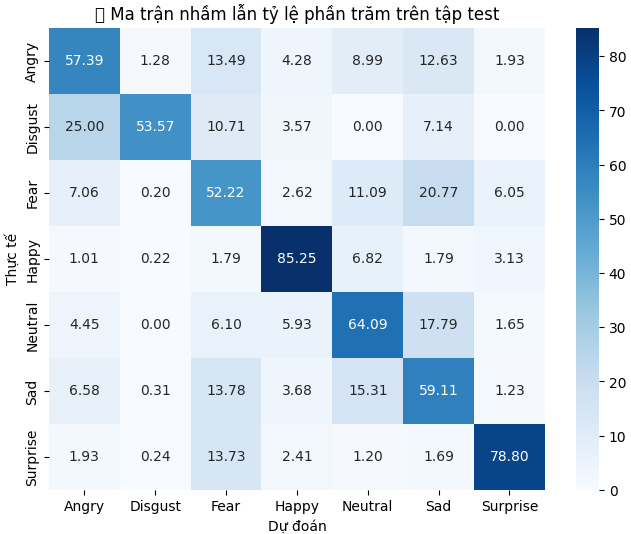
\includegraphics[width=1\textwidth]{img/confusionMatrixResnet18.png}
\caption{Ma trận nhầm lẫn phần trăm trên tập kiểm tra của mô hình ResNet18}
\label{fig:confusion-resnet18}
\end{figure}

Phân tích ma trận nhầm lẫn thể hiện tại Hình~\ref{fig:confusion-resnet18} cho thấy hiệu quả phân loại cảm xúc của mô hình ResNet18 trên tập kiểm tra. Mô hình đạt độ chính xác cao đối với các cảm xúc như \textit{Happy} (85.25\%) và \textit{Surprise} (78.80\%), tương đồng với các nghiên cứu trước đó về độ dễ nhận diện của các cảm xúc này qua biểu cảm khuôn mặt.

Ngược lại, các cảm xúc như \textit{Fear}, \textit{Sad} và \textit{Disgust} có xu hướng bị nhầm lẫn nhiều, đặc biệt là giữa các cặp có biểu hiện tương tự về hình thái học (ví dụ: \textit{Fear} và \textit{Sad}). Điều này cho thấy mô hình vẫn còn hạn chế trong việc tách biệt các đặc trưng tinh vi giữa các cảm xúc gần nhau về biểu cảm, một thách thức phổ biến trong nhận diện cảm xúc.

Những kết quả này gợi ý rằng việc cải thiện mô hình có thể tập trung vào việc xử lý mất cân bằng lớp, sử dụng dữ liệu tăng cường phù hợp và áp dụng kỹ thuật học sâu nâng cao để tăng cường khả năng phân biệt giữa các cảm xúc dễ gây nhầm lẫn.



% \begin{table}[H]
% \centering
% \rowcolors{2}{gray!20}{white}  % tô xen kẽ từ dòng 2
% \begin{tabular}{|>{\raggedright\arraybackslash}p{4cm}|l|l|l|l|}
% \hline
% \rowcolor{gray!40} \textbf{Tên kiến trúc} & \textbf{Accuracy (\%)} & \textbf{F1-score (\%)} & \textbf{Time infer (ms)} & \textbf{Size (MB)} \\
% \hline
% MobileNetV3Small & -- & -- & -- & -- \\
% ResNet18 & 67.23 & 67 & 3.44 & 42.73 \\
% MobileNetV3Small + FER2013 LLI  & -- & -- & -- & -- \\
% ResNet18 + FER2013 LLI  & 67.04 & 67 & 3.18 & 42.72 \\
% MobileNetV3Small +  FER2013 LLI +  adaptive augmentation& -- & -- & -- & -- \\
% ResNet18 +  FER2013 LLI +  adaptive augmentation& 67.48 & 67 & 2.91 & 42.72 \\
% \hline
% \end{tabular}
% \caption{Kết quả tổng thể}
% \end{table}




\subsection{Đánh giá, giải thích kết quả nghiên cứu}

\begin{table}[H]
\centering
\caption{Kết quả tổng thể của các mô hình}
\begin{tabular}{@{}>{\raggedright\arraybackslash}p{5cm}cccc@{}}
\toprule
\textbf{Tên kiến trúc} & \textbf{Accuracy (\%)} & \textbf{F1-score (\%)} & \textbf{Time infer (ms)} & \textbf{Size (MB)} \\ \midrule
MobileNetV3Small & 61.63 & 60 & 2.15 & 13.54 \\
ResNet18 & 67.23 & 67 & 3.44 & 42.73 \\
MobileNetV3Small + FER2013 LLI & 58.86 & 58 & 2.10 & 13.54 \\
ResNet18 + FER2013 LLI & 67.04 & 67 & 3.18 & 42.72 \\
MobileNetV3Small + FER2013 LLI + adaptive augmentation & 61.55 & 60 & 2.12 & 13.54 \\
ResNet18 + FER2013 LLI + adaptive augmentation & 67.48 & 67 & 2.91 & 42.72 \\ \bottomrule
\end{tabular}
\label{tab:overall-results}
\end{table}

Bảng trên tổng hợp các chỉ số chính của các mô hình thử nghiệm, bao gồm độ chính xác (Accuracy), F1-score, thời gian suy luận trên mỗi mẫu (Time inference), và kích thước mô hình (Size). 

\textbf{Nhận xét:}

\begin{itemize}
    \item \textbf{Hiệu suất nhận diện:} Mô hình ResNet18 cho kết quả vượt trội hơn hẳn MobileNetV3Small về độ chính xác và F1-score, chứng tỏ khả năng biểu diễn đặc trưng sâu sắc và hiệu quả hơn cho bài toán phân loại cảm xúc.
    
    \item \textbf{Ảnh hưởng của dữ liệu ánh sáng yếu (LLI):} Cả hai mô hình đều giảm nhẹ độ chính xác khi huấn luyện trên tập dữ liệu LLI, tuy nhiên sự sụt giảm này không đáng kể, đặc biệt là với ResNet18. Điều này cho thấy các kiến trúc mạng này có độ bền tốt với các biến đổi về điều kiện ánh sáng.
    
    \item \textbf{Tác động của kỹ thuật tăng cường dữ liệu thích ứng:} Khi kết hợp LLI với adaptive augmentation, độ chính xác của cả hai mô hình đều được cải thiện và gần đạt bằng hoặc vượt mức mô hình gốc. Đặc biệt với ResNet18, mức cải thiện rõ ràng và thời gian suy luận cũng giảm nhẹ, chứng tỏ kỹ thuật tăng cường dữ liệu giúp mô hình học được đặc trưng phong phú hơn và tăng khả năng tổng quát hóa.
    
    \item \textbf{Hiệu năng và kích thước mô hình:} MobileNetV3Small có lợi thế vượt trội về kích thước nhỏ gọn và thời gian suy luận nhanh hơn, phù hợp cho các ứng dụng thực tế trên thiết bị di động hoặc các hệ thống giới hạn tài nguyên. Ngược lại, ResNet18 với hiệu suất cao hơn đi kèm kích thước và thời gian suy luận lớn hơn, thích hợp cho các hệ thống yêu cầu độ chính xác cao.
\end{itemize}

\textbf{Kết luận:} 

Việc lựa chọn mô hình phụ thuộc vào mục tiêu ứng dụng cụ thể. Nếu ưu tiên độ chính xác và khả năng xử lý đa dạng điều kiện ánh sáng, ResNet18 là lựa chọn tối ưu. Trong khi đó, MobileNetV3Small phù hợp cho các ứng dụng cần tối ưu tài nguyên và tốc độ xử lý. Bên cạnh đó, áp dụng kỹ thuật tăng cường dữ liệu thích ứng được khuyến khích để cải thiện độ bền mô hình trong các môi trường ánh sáng thay đổi, giúp tăng khả năng nhận diện cảm xúc chính xác và ổn định hơn.




\subsection{Nêu ý nghĩa thực tiễn của nghiên cứu}
\begin{itemize}
    \item Cải thiện độ chính xác trong điều kiện ánh sáng yếu: Hệ thống nhận diện cảm xúc thường gặp khó khăn khi môi trường thiếu sáng (ví dụ: buổi tối, trong xe hơi, phòng họp mờ...). Nghiên cứu này giúp khắc phục vấn đề đó, tăng độ tin cậy và ổn định của mô hình trong điều kiện thực tế.
    \item Giảm chi phí phần cứng: Thay vì cần máy ảnh chất lượng cao để chụp rõ trong điều kiện ánh sáng kém, việc tăng cường ảnh bằng phần mềm cho phép sử dụng thiết bị giá rẻ, phù hợp với triển khai diện rộng.
\end{itemize}

% \subsection{Những hạn chế , đề xuất nghiên cứu tiếp theo}

% \subsubsection{Hạn chế}
% \begin{itemize}
%     \item Độ chỉnh xác tổng thể còn thấp
%     \item Còn nhầm lẫn giữa Disgust và Fear , Fear và Sad
%     \item Đôi khi việc áp dụng kĩ thuật tăng cường có thể làm cho thời gian suy luận ảnh lâu hơn
% \end{itemize}

% \subsubsection{Đề xuất nghiên cứu}
% \begin{itemize}
%     \item Ứng dụng các mô hình học sâu để tăng cường ảnh : Thử nghiệm các phương pháp tăng cường ảnh hiện đại như Deep Image Enhancement, GANs cho ảnh ánh sáng yếu để cải thiện chất lượng đầu vào.
%     \item Thu thập và mở rộng tập dữ liệu ánh sáng yếu : Xây dựng bộ dữ liệu đa dạng hơn về độ tuổi, giới tính, điều kiện ánh sáng, biểu cảm phức tạp hơn để huấn luyện và kiểm thử mô hình.
%     \item Phát triển mô hình nhẹ, tối ưu thời gian suy luận : Áp dụng kỹ thuật như quantization, pruning, hoặc thiết kế lại kiến trúc nhẹ (MobileNet, EfficientNet) để giảm độ trễ khi triển khai thực tế.
% \end{itemize}

